\documentclass[10pt]{article}
\usepackage{graphicx}
\usepackage{amssymb}
\usepackage[fleqn]{amsmath}
\usepackage{nccmath}
\usepackage{cases}
\usepackage{hyperref}
\usepackage{multicol}
\usepackage{pgfplots}
\usepackage{enumitem}
\pgfplotsset{compat=1.18}
\usepackage{float}
\usepackage{pdfpages}
\DeclareMathOperator*{\argmax}{argmax\,}
\DeclareMathOperator*{\argmin}{argmin\,}

\title{\bf Math 156: Problem Set 2}
\author{\bf Owen Jones}
\begin{document}
\maketitle
\begin{enumerate}
    \item $\displaystyle\underset{\mathbf{w}}{\argmax}P(\mathbf{w}|D,\alpha)=\underset{\mathbf{w}}{\argmax}P(D|\mathbf{w})P(\mathbf{w}|\alpha)\\
    =\underset{\mathbf{w}}{\argmax}(\prod_{n=1}^{N}\frac{\sqrt{\beta}}{\sqrt{2\pi}}e^{-\frac{\beta}{2}{(t_n-y(x_n,\mathbf{w}))}^2}){(\frac{\alpha}{2\pi})}^{\frac{(M+1)}{2}}e^{-\frac{\alpha}{2}\mathbf{w}^\top\mathbf{w}}\\
    =\underset{\mathbf{w}}{\argmax}\log((\prod_{n=1}^{N}\frac{\sqrt{\beta}}{\sqrt{2\pi}}e^{-\frac{\beta}{2}{(t_n-y(x_n,\mathbf{w}))}^2}){(\frac{\alpha}{2\pi})}^{\frac{(M+1)}{2}}e^{-\frac{\alpha}{2}\mathbf{w}^\top\mathbf{w}})\\
    =\underset{\mathbf{w}}{\argmax}\frac{N}{2}\log(\frac{\beta}{2\pi})+\frac{M+1}{2}\log(\frac{\alpha}{2\pi})-\frac{\beta}{2}\sum_{n=1}^{N}{(t_n-y(x_n,\mathbf{w}))}^2-\frac{\alpha}{2}\mathbf{w}^\top\mathbf{w}\\
    =\underset{\mathbf{w}}{\argmax}-\frac{\beta}{2}\sum_{n=1}^{N}{(t_n-y(x_n,\mathbf{w}))}^2-\frac{\alpha}{2}\mathbf{w}^\top\mathbf{w}\\
    =\underset{\mathbf{w}}{\argmin}\frac{\beta}{2}\sum_{n=1}^{N}{(t_n-y(x_n,\mathbf{w}))}^2+\frac{\alpha}{2}\mathbf{w}^\top\mathbf{w}$\\
    which is the minimizer of our desired function.\\
    The MAP approach adds a regularizer term to MLE approach.
    \item Suppose for the sake of contradiction $\{\mathbf{x}_n\}$ and $\{\mathbf{y}_n\}$ are linearly separable, but there exists a point $\mathbf{z}$ where the two convex hulls intersect.\\
    Let $\displaystyle\mathbf{z}=\sum_{n}\alpha_n\mathbf{x}_n=\sum_{n}\beta_n\mathbf{y}_n$.\\
    It follows $\displaystyle\mathbf{w}^\top\mathbf{z}+w_0=\mathbf{w}^\top(\sum_{n}\alpha_n\mathbf{x}_n)+w_0=\mathbf{w}^\top(\sum_{n}\beta_n\mathbf{y}_n)+w_0$\\
    $\displaystyle\mathbf{w}^\top(\sum_{n}\alpha_n\mathbf{x}_n)+w_0=\sum_{n}\alpha_n(\mathbf{w}^\top\mathbf{x}_n)+w_0$ because $\alpha_n$ is a scalar quantity.\\
    Using $\displaystyle\sum_{n}\alpha_n=1$, we obtain $\displaystyle\sum_{n}\alpha_n(\mathbf{w}^\top\mathbf{x}_n)+w_0=\sum_{n}\alpha_n(\mathbf{w}^\top\mathbf{x}_n+w_0)$.\\
    Thus, we have $\displaystyle\sum_{n}\alpha_n(\mathbf{w}^\top\mathbf{x}_n+w_0)=\sum_{n}\beta_n(\mathbf{w}^\top\mathbf{y}_n+w_0)$.
    However, this is impossible for all $\alpha_n,\beta_n\ge 0$ because by assumption $\mathbf{w}^\top\mathbf{x}_n+w_0>0,\mathbf{w}^\top\mathbf{y}_n+w_0<0$.
    Hence, $\{\mathbf{x}_n\}$ and $\{\mathbf{y}_n\}$ are not linearly separable.\\

    Suppose for the sake of contradiction there exists a point $\mathbf{z}$ where the two convex hulls intersect, but the convex hulls are linearly separable.\\
    It follows there exists a vector $\vec{\mathbf{w}}$ and scalar $w_0$ s.t $\mathbf{w}^\top\mathbf{x}_n+w_0>0$ and $\mathbf{w}^\top\mathbf{y}_n+w_0<0$.
    Since $\mathbf{z}$ lies on the intersection of the two convex hulls, $\displaystyle\mathbf{z}=\sum_{n}\alpha_n\mathbf{x}_n=\sum_{n}\beta_n\mathbf{y}_n$.
    However, $\displaystyle\sum_{n}\alpha_n(\mathbf{w}^\top\mathbf{x}_n+w_0)=\sum_{n}\mathbf{w}^\top(\alpha_n\mathbf{x}_n)+w_0=\sum_{n}\mathbf{w}^\top\mathbf{z}+w_0>0$ and $\displaystyle\sum_{n}\beta_n(\mathbf{w}^\top\mathbf{y}_n+w_0)=\sum_{n}\mathbf{w}^\top(\beta_n\mathbf{y}_n)+w_0=\sum_{n}\mathbf{w}^\top\mathbf{z}+w_0<0$ which is clearly a contradiction.
    Hence, the two convex hulls do not intersect.
    \item See the function SGD in the attached code
    \item For the purpose of this problem, I chose to use sklearn's MinMax scaler on the features in the dataset. 
    The parameters I chose for my SGD classification model were to RSME less than 0.1 as the termination conditon, $100,000$ max iterations, $10\%$ of total population as the batch size, and a learning rate of $0.005$. 
    I used a train, validation, test split of $60\%$, $20\%$, and $20\%$.
    The model performed very wel on the test set (See classification report). Precision, recall, and f-1 score were all in the low to mid $90s$ except for the the recall on class $0$. Thus, the ration of True negatives to total number of negatives is slightly worse than the other metrics.
    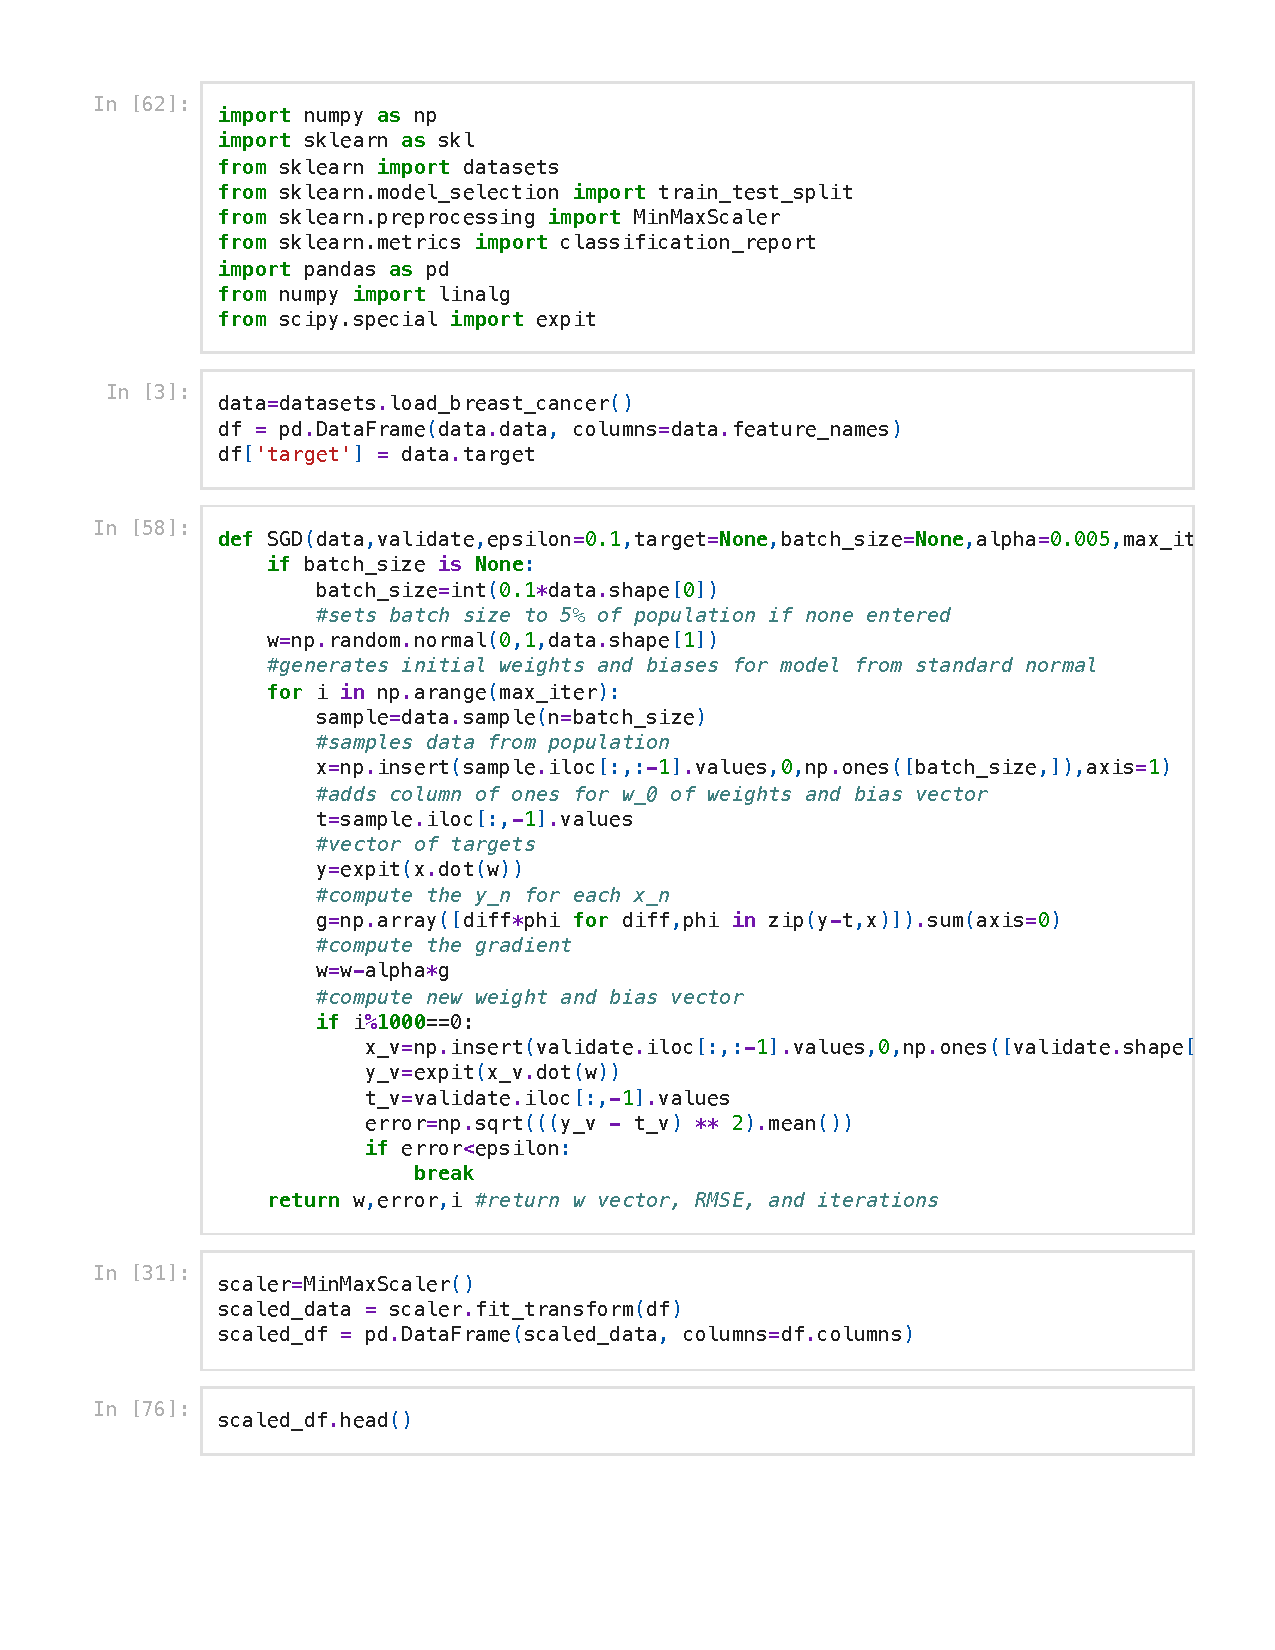
\includepdf[pages=-]{Homework_2_Math_156.pdf}
\end{enumerate}
\end{document}